\chapter{Ornamentation HMM}\label{ch:hmm-ornamentation}
Il primo modello di Markov aggiunge una sola nota per battuta per le linee melodiche di contralto, tenore e basso, questa è una semplificazione rispetto ai corali reali di Bach che possono invece presentare quattro note per battuta come accade per la linea melodica del soprano. Questo problema viene risolto addestrando un secondo modello di Markov nascosto in cui gli stati visibili rappresentano quanto le tre linee musicali crescono o decrescono tra una battuta ed un altra, mentre gli stati nascosti rappresentano di quanto dovrebbe essere alzato o abbassato uno degli ultimi tre quarti della battuta. 
\begin{figure}[H]
	\centering
	\caption{(a) stati nascosti, (b) stati visibili}
	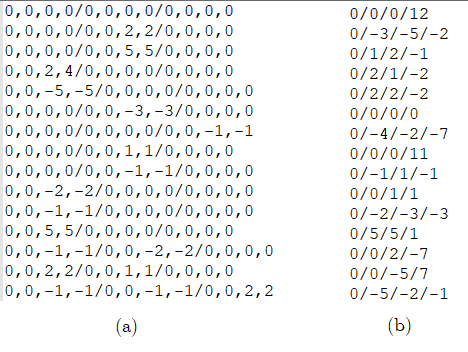
\includegraphics{figures/hid-vis-orn.png}
	\label{hid-vis-orn}
\end{figure}
\noindent
Ad esempio facendo riferimento all'ultima riga dell'immagine in figura vediamo che per una battuta in cui, nella battuta successiva, il contralto scende di 5 semitoni, il tenore scende di 2 semitoni e il basso scende di due semitoni andrà a generare le tre linee melodiche in cui la terza e la quarta nota sono rispettivamente abbassate di un semitono per contralto e tenore, ed alzate di due semitoni per il basso.
\section{Training}
Anche in questo caso prima del training viene effettuata una parte di preprocessing per ottenere gli stati visibili e nascosti, il training del modello viene eseguito esattamente come descritto nel capitolo precedente.
\section{Testing}
Anche in questo caso si opera nella stessa identica maniera descritta precedentemente, i risultati in termini di accuratezza vengono mostrati in tabella.
\section{Ricostruzione dei risultati}
Per ricostruire i risultati è stato necessario aggiungere uno script non presente nel repository originale in grado modificare il file musicale costruito dal modello di Markov precedente in accordo con la modifica di semitono delle linee melodiche.
\section{Genearazione del file MIDI}
Una volta integrati i risultati dei due modelli è possibile costruire i file MIDI utilizzando lo stesso script relativo al modello precedente.
\section{Ornamentazione di musica moderna}
Non è invece possibile eseguire il task di ornamentazione della musica moderna, questo è dovuto al fatto che i file costruiti da noi contengono esclusivamente informazione relativa alla melodia del soprano e come tale non è possibile costruire gli stati visibili e nascosti richiesti dal modello per funzionare.
  